\section {Backend}

The client agreed on having an Erlang NetInf NRS. The backend product implements the, as of writing, current draft of the NetInf Protocol\cite{netinfproto}.  in a purely functional language. The product promises a high level of scalability and fault-tolerance. The client initially asked for only the NRS as a product however the backend team was able to complete the initial product in a timely manner, allowing for applications of this network technology to be explored. 


\subsection {Erlang NetInf Name Resolution Service}
The first of the two deliverables from the backend team to the client. The Erlang NetInf NRS provides a new way to organize and retrieve data on the Internet. Based on an initial NetInf NRS protocol draft from development teams such as SAIL and Ericsson Research. This product allows for flexibility and extension of the existing protocol.

Erlang's concept of modularization allowed the team to break up the NRS functionality into distinctive convergence layers, runtime database switching, and even allow for a proof-of-concept data streaming client/protocol. 

\subsection{NetInf Video Streaming Client/Protocol}

The last of the deliverables from the backend team. The HTML interface requested a proof-of-concept video streaming protocol and client which lies on top of the Erlang NetInf NRS technology. The streaming protocol is a completely new addition to the NetInf draft. The team developed a way to utilize the code and transporting mechanism of the first product in order to stream video content. Along with the protocol outlined below, the team has created a http interface 'client' which allows the user to see the streaming protocol in action in addition to accessing the NRS functionality. This particular product was not specified in the initial conversations with the client in September, but was added late in the development cycle and is a proof-of-concept.

\subsubsection{First Implementation}
In addition to normal NRS functionality, a HTTP transfer-dispatcher had to be implemented in order to transfer of chunks between clients. The streaming works by clients subscribing to a stream from a specific NRS. Once connected the client, with a constant interval will ask the NRS where to find these chunks. All the chunks are transferred via the transfer-dispatcher.
The playback of the video chunks is done by polling the local NRS, this implies that every client has its own NetInf node running. See figure \ref{fig:stream-seqorgmod}. The benefit of using this approach is that only one NDO containing the filename has to be published. The receiver can then derive the chunks locations, by appending the chunk number to the end of the locators provided in the filename NDO.

\begin{figure}[h!]
	\centering
		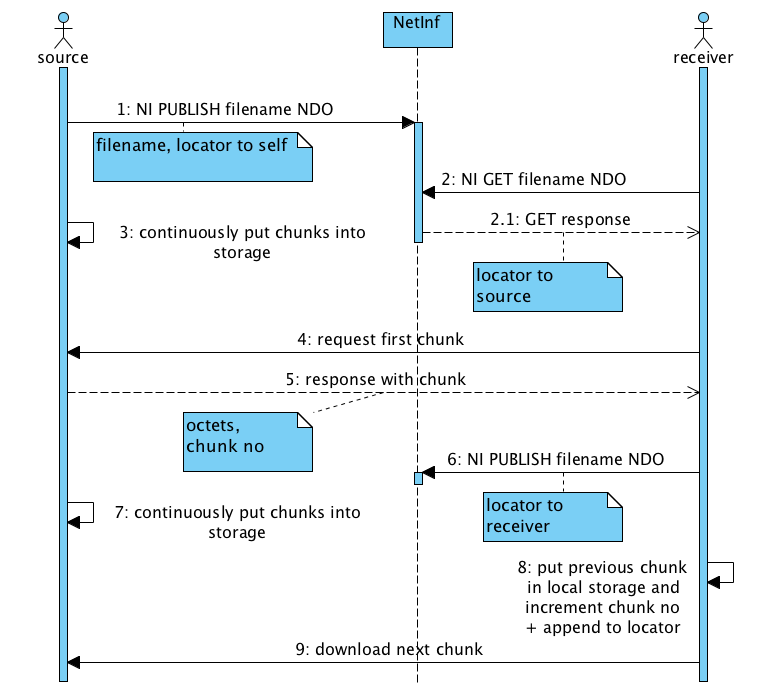
\includegraphics[width=0.75\textwidth]{./img/sequence_diagram_streaming_orgmod.png}
    	\caption{Original/Modified Chunked Data Transfer}
	\label{fig:stream-seqorgmod}
\end{figure}

\subsubsection{Modified NetInf Streaming}
Due to a request from the client a more true NetInf implementation of streaming was implemented. Instead of using the transfer-dispatcher between the client nodes a workaround was added that disabled content validation, this resulted in fetching of chunks via NetInf messages. The polling logic is still the same as first implementation, seen in figure \ref{fig:stream-seqorgmod}. Instead of using ordinary HTTP locators, the receiver is required to modify the \textit{NetInf GET requests} to get the chunks. This is done by replacing the hash algorithm with the custom hash name \textit{demo}. For example to get the first chunk of \textit{ni:///sha-256;abc}, the request should contain \textit{ni:///demo;abc1}. The HTTP transfer-dispatcher is still used to transfer the chunks to the HTML-interface.

\subsubsection{Pure NetInf Streaming}
To be able to evaluate the modified NetInf streaming another implementation was added. This implementation uses NetInf searches and gets for chunks. See Figure~\ref{fig:stream-seq-pure}. In this implementation the stream source is required to publish each chunk to the NRS, and modify the NDO metadata with the stream name and stream chunk number. The receiver is then required to search for each chunk to find it. 

\begin{figure}[h!]
	\centering
		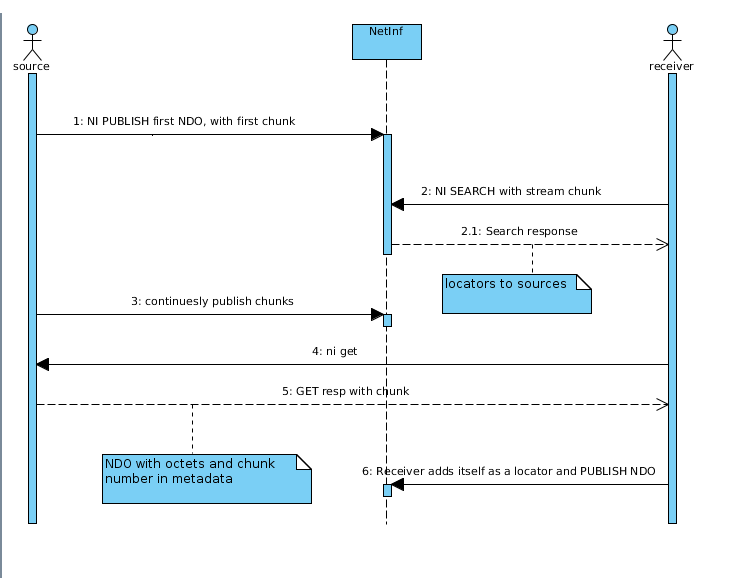
\includegraphics[width=0.75\textwidth]{./img/sequence_diagram_pure_streaming.png}
    	\caption{Chunked Data Transfer With Pure NetInf}
	\label{fig:stream-seq-pure}
\end{figure}

\subsubsection{Streaming Frontend}
To merge the chunks, a simple HTML5 frontend was created. HTML was chosen to make the player platform independent.
In both implementations the player starts a JavaScript that continuously polls the local NetInf node for the chunks through the HTTP dispatcher.
The difference is that the pure NetInf player uses the NRS search to build the playlist, while the modified NetInf version only increases the chunk number.
